% Appendix E: supplementary tables and figures moved out of the main body to keep it within
% the 50-page limit. Content unchanged; sources as noted in each chapter file.
\chapter{Supplementary Tables and Figures}
\label{app:supp}

This appendix holds tables and figures that support the main chapters. Each is referred to
from the chapter named in its section heading.

\section{Requirements and system analysis}

\begin{table}[H]
\centering
\caption{Stakeholders of StripCheck and what each needs from the system}
\label{tab:req-stakeholders}
\small\renewcommand{\_}{\textunderscore\allowbreak}
\begin{tabularx}{\linewidth}{@{}>{\raggedright\arraybackslash}p{3.3cm} >{\raggedright\arraybackslash}X >{\raggedright\arraybackslash}p{2.6cm}@{}}
\toprule
\textbf{Role} & \textbf{Need} & \textbf{Requirement} \\ \midrule
Patient or caregiver holding a pack (primary user) & A clear answer on whether this batch is listed, with the list and month, and a next step that does not cause harm & FR1, FR5, NFR4 \\
Community pharmacist & A result that names the listed batch, the list month and the source row, so that the claim can be checked against the CDSCO list & FR5, NFR5 \\
Manufacturer or marketer named on a list & No alarm on a different batch or on a brand as a whole; a false alarm on a sibling batch harms a product that was not listed & FR3, FR4, NFR4 \\
CDSCO and state drug-testing laboratories (publishers of the lists) & Correct attribution of every alert, polite access to the portal, and no claim that the tool is an official service & FR6, NFR5, NFR8 \\
Project team (operators and evaluators) & Reproducible data sync, step-level traces and an evaluation command with a stated decision rule & FR8, FR10, NFR6 \\
\bottomrule
\end{tabularx}
\end{table}

\section{Agent design}

\begin{table}[H]
\centering
\caption{Agentic patterns used in StripCheck and the alternatives rejected}
\label{tab:design-patterns}
\small\renewcommand{\_}{\textunderscore\allowbreak}
\begin{tabularx}{\linewidth}{@{}>{\raggedright\arraybackslash}p{2.6cm} >{\raggedright\arraybackslash}p{2.2cm} >{\raggedright\arraybackslash}X >{\raggedright\arraybackslash}p{2.9cm}@{}}
\toprule
\textbf{Pattern} & \textbf{Where} & \textbf{Reason} & \textbf{Alternative rejected} \\ \midrule
Bounded tool loop (plan, act, observe)~\cite{yao2023react} & Investigator & Each step is a logged tool call; the loop has a step cap and runs without a model & Unbounded loop driven by the model \\
Model as advisor or tool picker under rule-computed allowed tools~\cite{kambhampati2024llmmodulo} & Planner: (b), (c); agent mode & A 3B local model chooses only among allowed actions or tools; rules check and replace its choice & Model plans every step with all tools \\
Corrective retrieval with a grader & Exact and variant search, grade & A misread batch is expected; an empty exact search triggers a bounded look-alike search, and grading removes collisions & Single exact lookup (the baseline of Chapter~\ref{ch:eval}) \\
Record linkage~\cite{fellegi1969theory} & Grader & A shared batch string is not identity; product, dates and maker must agree & Embedding similarity over alert text \\
External verifier and one bounded revision (reflection)~\cite{huang2024cannot} & Verifier, \texttt{reflect} & Hard rules re-check the draft; \texttt{reflect} allows one more question or abstention & Model self-critique~\cite{madaan2023selfrefine,shinn2023reflexion} \\
Vision fallback with confirmation & Perception & A local vision model reads the batch line when OCR cannot; the person confirms before the value counts & Vision value used as evidence \\
Human-in-the-loop interrupt & \texttt{ask\_user} & Only the person holding the pack can read the printed character & Yes/no confirm button; fully automatic alarm \\
Abstention~\cite{chow1970reject,geifman2017selective} & \CANTV{} & Weak evidence ends in an explicit ``more evidence is needed'' & Forced choice between alarm and \NLISTED \\
Hand-offs and a monitor & Four agents; background lane & Message records between agents; a scheduled cycle of sync, re-check and notification & Free multi-agent conversation~\cite{wu2023autogen} \\
\bottomrule
\end{tabularx}
\end{table}


\begin{table}[H]
\centering
\caption{Fields of the agent state saved after every run}
\label{tab:design-state}
\small\renewcommand{\_}{\textunderscore\allowbreak}
\begin{tabularx}{\linewidth}{@{}>{\raggedright\arraybackslash}p{4.1cm} >{\raggedright\arraybackslash}X@{}}
\toprule
\textbf{Field} & \textbf{Content} \\ \midrule
\texttt{history} & Ordered steps: action, source, summary, time in ms, and where present the thought, the prior used and the verifier result \\
\texttt{asks}, \texttt{declined} & Number of questions asked so far; question kinds the person answered with ``Can't tell'' \\
\texttt{batch\_evidence} & How the batch is known: \texttt{qr}, \texttt{ocr}, \texttt{dual\_read}, \texttt{user\_typed}, \texttt{user\_confirmed} or \texttt{none} \\
\texttt{provenance} & Source of each pack field (\texttt{qr}, \texttt{ocr}, \texttt{ocr\_enh}, \texttt{carton}, \texttt{user}) \\
\texttt{candidates}, \texttt{pending} & Graded candidates with status and per-field evidence; the open question, if any \\
\texttt{rejected\_keys}, \texttt{confirmed\_keys}, \texttt{conflict\_ids} & Effects of earlier answers that later runs must respect \\
\texttt{exact\_searched}, \texttt{variants\_searched}, \texttt{truncated} & Search coverage flags that the verifier checks for \NLISTED \\
\texttt{planner}, \texttt{decisions}, \texttt{session} & Planner mode, the source of each branch-point decision, and the trace identifiers \\
\texttt{messages}, \texttt{observations}, \texttt{revisions} & Hand-off messages (at most 24), tool observations carried into later turns, and the number of revisions used (at most 1) \\
\texttt{vision}, \texttt{vision\_calls}, \texttt{photos} & The pending vision reading with its crop, and the vision calls (at most 2) and extra photos (at most 1) used \\
\bottomrule
\end{tabularx}
\end{table}

\begin{table}[H]
\centering
\caption{Loops and limits in the design and how each terminates}
\label{tab:design-bounds}
\footnotesize\renewcommand{\_}{\textunderscore\allowbreak}
\begin{tabularx}{\linewidth}{@{}>{\raggedright\arraybackslash}p{3.2cm} >{\raggedright\arraybackslash}p{3.0cm} >{\raggedright\arraybackslash}X@{}}
\toprule
\textbf{Loop or limit} & \textbf{Bound} & \textbf{On reaching it} \\ \midrule
Steps per check & 16 (\texttt{MAX\_STEPS}) & No new question after 12 steps; at 13 steps the run abstains; R6 downgrades any draft above 16 \\
Questions per check & 2 (\texttt{MAX\_ASKS}) & The pending candidate is drafted as \CANTV{} with its reason \\
Variant search & 2 substitutions, 2{,}000 keys & The search stops at the limit and returns what it found \\
Candidates graded & 20 & More matches end in \CANTV{} (``too many records share this batch'') \\
Verifier send-back, \texttt{reflect} & 1 (\texttt{MAX\_REVISIONS}) & R4 return of an early model draft, or one revision (one more question) after another violation; then \CANTV \\
Agent turns, observations & 16 steps; last 8 observations of 1{,}500 characters each; 24 hand-off messages & Rule choice with source \texttt{rules(fallback)} \\
Vision read & 2 calls, 1 extra photo, 30\,s default timeout (1 to 60\,s) & The person is asked to type the batch; a timeout does not start the 30\,s skip \\
Monitor cycle & Every 6\,h by default, first run 30\,s after start, back-off up to 24\,h, 200 cycles kept & A failed cycle is recorded and retried later; checks are unaffected \\
Model call & 2 attempts, 15\,s each (configurable 1 to 90\,s, at most 45 used) & Rule suggestion with source \texttt{rules(fallback)}; model skipped for 30\,s after a connection error; loopback endpoint only \\
Photo read & 60\,s per photo, 30\,s per reader, 20\,s barcode, 1 re-read & Empty fields; the person is asked to type the batch \\
Upload & 15\,MB, 24 million pixels, 2{,}400\,px per side & Larger uploads are refused; larger images are shrunk \\
Portal request & $\ge$1.5\,s apart, 20\,s timeout, 3 attempts, 16\,MB & Sync stops; the existing index stays in use \\
Tracing and streaming & 0.25\,s probe, 3\,s export; queue of 2{,}048 events, 15\,s heartbeat & Spans are skipped; a tracer failure never fails a check \\
\bottomrule
\end{tabularx}
\end{table}

\section{Implementation}

\begin{table}[H]
\centering
\caption{Technology stack and installed versions}
\label{tab:stack}
\footnotesize
\begin{tabularx}{\linewidth}{@{}>{\raggedright\arraybackslash}p{2.6cm} >{\raggedright\arraybackslash}p{5.2cm} >{\raggedright\arraybackslash}X@{}}
\toprule
\textbf{Layer} & \textbf{Choice (version)} & \textbf{Reason} \\ \midrule
Language & Python 3.12.7 & One language for engine, ingest and evaluation \\
Agent engine & Own bounded loop, \texttt{core/investigator.py} & Small, testable, resumable (decision D18) \\
Storage & SQLite (standard library), WAL mode & One local file for alerts, checks, memory \\
API server & FastAPI 0.162.0, Uvicorn 0.54.0, Pydantic 2.14.1 & Streams steps and questions as server-sent events \\
Text reading & RapidOCR 3.10.0, PP-OCRv6-small on ONNX Runtime 1.31.1; Apple Vision on macOS & Local, CPU only, no download at run time \cite{rapidai2021rapidocr,du2020ppocr} \\
Barcodes & zxing-cpp 3.1.1; OpenCV headless 4.14.0.94 & GS1 payloads carry a check digit \\
Images & Pillow 13.0.0, pillow\_heif 1.8.1 & Validation, resizing, HEIC photos \\
Fuzzy matching & RapidFuzz 3.14.6 & Maker similarity in grading \\
Local LLM (optional) & Ollama 0.17.7, \texttt{qwen2.5:3b}; \texttt{qwen2.5vl:3b} for vision & JSON-schema output and tool calls from local models \cite{ollama2026structured} \\
Tracing (optional) & OpenTelemetry SDK 1.45.1; Arize Phoenix 21.0.0 & Standard spans, viewed locally \cite{otel2026genai,arize2026openinference} \\
Clients & React 19.3.1, TypeScript 6.0.3, Vite 8.3.5; SwiftUI (iOS 17) & Step timeline, question cards, camera \\
Tests & pytest 9.1.1; Vitest 5.0.5 & Offline by default \\
\bottomrule
\end{tabularx}
\end{table}

\begin{table}[H]
\centering
\caption{Verifier rules as implemented}
\label{tab:verifier}
\footnotesize
\begin{tabularx}{\linewidth}{@{}l >{\raggedright\arraybackslash}X@{}}
\toprule
\textbf{Rule} & \textbf{Condition checked on the draft and the stored state} \\ \midrule
R1 & The label is one of the four verdicts \\
R2 & An alarm needs an accepted candidate with an exact or confirmed batch, batch evidence from QR, two agreeing reads or the person, a product match (or a partial match with dates and maker), no field mismatch, and equal batch keys \\
R3 & \SFAKE{} only for a spurious entry; \FLAGGED{} only for NSQ, misbranded or adulterated entries \\
R4 & \NLISTED{} needs a grounded batch, both searches run, no pending or accepted candidate, loaded data, no truncation \\
R5 & An alarm cites the entry with a source URL or SHA-256; no text contains a banned phrase \\
R6 & At most 16 steps and 2 questions \\
R7 & Outside \CANTV, no candidate has an unresolved date conflict \\
R8 & Outside \CANTV, every field used has a grounded source (person, OCR, QR, enhanced OCR, carton) \\
R9 & \NLISTED{} states the lists loaded and the latest list month \\
R10 & The verdict language is a reviewed one (English) \\
\bottomrule
\end{tabularx}
\end{table}


\begin{table}[H]
\centering
\caption{Tools used by the agent and by the background pipeline}
\label{tab:tools}
\footnotesize
\begin{tabularx}{\linewidth}{@{}>{\raggedright\arraybackslash}p{2.7cm} >{\raggedright\arraybackslash}X >{\raggedright\arraybackslash}p{4.3cm}@{}}
\toprule
\textbf{Tool (module)} & \textbf{Input $\rightarrow$ output} & \textbf{Bounds and errors} \\ \midrule
\texttt{decode\_qr} (\texttt{pack\_tools}) & image $\rightarrow$ batch, dates, GTIN from GS1 payload & Separate process, 20\,s; failure gives no fields \\
\texttt{ocr\_read} (\texttt{pack\_tools}) & image $\rightarrow$ text lines with box, score, engine & 30\,s per reader, 60\,s per photo; failure gives no lines \\
\texttt{extract\_fields} & lines, QR fields $\rightarrow$ batch, product, brand, dates, maker with provenance & Empty field when no label matches \\
\texttt{search\_exact} (\texttt{matching}) & batch key $\rightarrow$ alert rows with that key & At most 21 rows \\
\texttt{search\_variants} & batch key, prior $\rightarrow$ rows at look-alike keys, substitutions, score & $\le 2$ substitutions, $\le 2{,}000$ keys, $\le 21$ rows \\
\texttt{grade} & alert row, pack fields $\rightarrow$ evidence per field and a status & Deterministic; unknown stays unknown \\
\texttt{ask\_user} (\texttt{templates}) & kind, candidate $\rightarrow$ question payload; check pauses & At most 2 per check; ``Can't tell'' offered \\
\texttt{draft\_verdict} & label, fields, entry $\rightarrow$ templated verdict with citation & Verified; failure gives \CANTV \\
\texttt{sync}, \texttt{ingest} & portal months $\rightarrow$ snapshots $\rightarrow$ validated rows & 1.5\,s spacing, 3 attempts; failure keeps index \\
\texttt{read\_\allowbreak with\_\allowbreak vision} (\texttt{llm}) & batch-line crop or photo $\rightarrow$ batch, dates, confidence, note & 2 per check, 30\,s default; the reading is used only after a \texttt{confirm\_reading} yes; failure leads to a typing question \\
\texttt{request\_photo} & kind (batch zoom, second angle, carton) $\rightarrow$ re-run perception on the upload & 1 per check; the person may decline \\
\texttt{reflect}, \texttt{downgrade} & verifier violations $\rightarrow$ one more question or abstention & At most 1 revision per check \\
\texttt{recheck\_cabinet} & saved packs $\rightarrow$ verdicts, notifications & Same investigator, no questions \\
\texttt{run\_cycle} (\texttt{monitor}) & schedule $\rightarrow$ sync decision, sync, re-check, notifications & Back-off after failures; never affects a check \\
\bottomrule
\end{tabularx}
\end{table}

\begin{figure}[H]
\centering
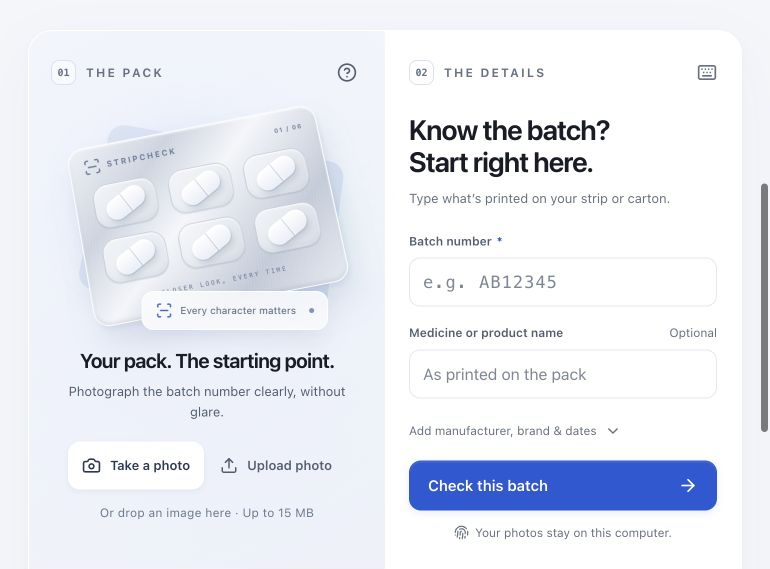
\includegraphics[width=\textwidth]{fig_ui_check_crop.png}
\caption{Start of a check in the web client: photo capture or upload (left) and typed batch details (right). Screenshot of the local client at 770 by 569 pixels.}
\label{fig:ui-check}
\end{figure}

\section{Observability and evaluation}

\begin{table}[H]
\centering
\caption{Headline metrics on the evaluation set (seed~7, $n=60$, final run), with Wilson 95\% intervals below the rates. Source: \texttt{paper/generated/results.tex}.}
\label{tab:eval-results-full}
\scriptsize
\setlength{\tabcolsep}{2.5pt}
\renewcommand{\arraystretch}{1.12}
\begin{tabularx}{\linewidth}{@{}>{\raggedright\arraybackslash}p{2.9cm} cccc@{}}
\toprule
\textbf{Metric} & \textbf{Baseline (lookup)} & \textbf{Agent (rules)} & \textbf{Agent (hybrid)} & \textbf{Agent (tools)} \\
\midrule
\multicolumn{5}{@{}l}{\textit{HITL = oracle (a person answers every question)}} \\
Hit recall & \res{ResBaseOracleHitRecall} (\res{ResBaseOracleHitRecallK}) & \res{ResRulesOracleHitRecall} (\res{ResRulesOracleHitRecallK}) & \res{ResHybridOracleHitRecall} (\res{ResHybridOracleHitRecallK}) & \res{ResLLMOracleHitRecall} (\res{ResLLMOracleHitRecallK}) \\
 & \res{ResBaseOracleHitRecallCI} & \res{ResRulesOracleHitRecallCI} & \res{ResHybridOracleHitRecallCI} & \res{ResLLMOracleHitRecallCI} \\
Hit recall, clean and QR & \res{ResBaseOracleHitRecallCleanQR} (\res{ResBaseOracleHitRecallCleanQRK}) & \res{ResRulesOracleHitRecallCleanQR} (\res{ResRulesOracleHitRecallCleanQRK}) & \res{ResHybridOracleHitRecallCleanQR} (\res{ResHybridOracleHitRecallCleanQRK}) & \res{ResLLMOracleHitRecallCleanQR} (\res{ResLLMOracleHitRecallCleanQRK}) \\
Type accuracy & \res{ResBaseOracleTypeAcc} (\res{ResBaseOracleTypeAccK}) & \res{ResRulesOracleTypeAcc} (\res{ResRulesOracleTypeAccK}) & \res{ResHybridOracleTypeAcc} (\res{ResHybridOracleTypeAccK}) & \res{ResLLMOracleTypeAcc} (\res{ResLLMOracleTypeAccK}) \\
False-alarm rate, all not listed & \res{ResBaseOracleFAR} (\res{ResBaseOracleFARK}) & \res{ResRulesOracleFAR} (\res{ResRulesOracleFARK}) & \res{ResHybridOracleFAR} (\res{ResHybridOracleFARK}) & \res{ResLLMOracleFAR} (\res{ResLLMOracleFARK}) \\
 & \res{ResBaseOracleFARCI} & \res{ResRulesOracleFARCI} & \res{ResHybridOracleFARCI} & \res{ResLLMOracleFARCI} \\
False-alarm rate, collisions & \res{ResBaseOracleFARCollision} (\res{ResBaseOracleFARCollisionK}) & \res{ResRulesOracleFARCollision} (\res{ResRulesOracleFARCollisionK}) & \res{ResHybridOracleFARCollision} (\res{ResHybridOracleFARCollisionK}) & \res{ResLLMOracleFARCollision} (\res{ResLLMOracleFARCollisionK}) \\
False-alarm rate, siblings & \res{ResBaseOracleFARSibling} (\res{ResBaseOracleFARSiblingK}) & \res{ResRulesOracleFARSibling} (\res{ResRulesOracleFARSiblingK}) & \res{ResHybridOracleFARSibling} (\res{ResHybridOracleFARSiblingK}) & \res{ResLLMOracleFARSibling} (\res{ResLLMOracleFARSiblingK}) \\
Abstention rate & \res{ResBaseOracleAbstain} (\res{ResBaseOracleAbstainK}) & \res{ResRulesOracleAbstain} (\res{ResRulesOracleAbstainK}) & \res{ResHybridOracleAbstain} (\res{ResHybridOracleAbstainK}) & \res{ResLLMOracleAbstain} (\res{ResLLMOracleAbstainK}) \\
Overall accuracy & \res{ResBaseOracleAccuracy} (\res{ResBaseOracleAccuracyK}) & \res{ResRulesOracleAccuracy} (\res{ResRulesOracleAccuracyK}) & \res{ResHybridOracleAccuracy} (\res{ResHybridOracleAccuracyK}) & \res{ResLLMOracleAccuracy} (\res{ResLLMOracleAccuracyK}) \\
 & \res{ResBaseOracleAccuracyCI} & \res{ResRulesOracleAccuracyCI} & \res{ResHybridOracleAccuracyCI} & \res{ResLLMOracleAccuracyCI} \\
Questions / steps per pack & \res{ResBaseOracleQuestions} / \res{ResBaseOracleSteps} & \res{ResRulesOracleQuestions} / \res{ResRulesOracleSteps} & \res{ResHybridOracleQuestions} / \res{ResHybridOracleSteps} & \res{ResLLMOracleQuestions} / \res{ResLLMOracleSteps} \\
Latency median / mean / p95 (s) & \res{ResBaseOracleLatMedian} / \res{ResBaseOracleLatMean} / \res{ResBaseOracleLatPNinetyFive} & \res{ResRulesOracleLatMedian} / \res{ResRulesOracleLatMean} / \res{ResRulesOracleLatPNinetyFive} & \res{ResHybridOracleLatMedian} / \res{ResHybridOracleLatMean} / \res{ResHybridOracleLatPNinetyFive} & \res{ResLLMOracleLatMedian} / \res{ResLLMOracleLatMean} / \res{ResLLMOracleLatPNinetyFive} \\
LLM steps / fallback steps & \res{ResBaseOracleLLMSteps} / \res{ResBaseOracleFallbackSteps} & \res{ResRulesOracleLLMSteps} / \res{ResRulesOracleFallbackSteps} & \res{ResHybridOracleLLMSteps} / \res{ResHybridOracleFallbackSteps} & \res{ResLLMOracleLLMSteps} / \res{ResLLMOracleFallbackSteps} \\
Safety violations & \res{ResBaseOracleSafety} & \res{ResRulesOracleSafety} & \res{ResHybridOracleSafety} & \res{ResLLMOracleSafety} \\
\midrule
\multicolumn{5}{@{}l}{\textit{HITL = none (every question skipped)}} \\
Hit recall & \res{ResBaseSkipHitRecall} (\res{ResBaseSkipHitRecallK}) & \res{ResRulesSkipHitRecall} (\res{ResRulesSkipHitRecallK}) & \res{ResHybridSkipHitRecall} (\res{ResHybridSkipHitRecallK}) & \res{ResLLMSkipHitRecall} (\res{ResLLMSkipHitRecallK}) \\
 & \res{ResBaseSkipHitRecallCI} & \res{ResRulesSkipHitRecallCI} & \res{ResHybridSkipHitRecallCI} & \res{ResLLMSkipHitRecallCI} \\
Hit recall, clean and QR & \res{ResBaseSkipHitRecallCleanQR} (\res{ResBaseSkipHitRecallCleanQRK}) & \res{ResRulesSkipHitRecallCleanQR} (\res{ResRulesSkipHitRecallCleanQRK}) & \res{ResHybridSkipHitRecallCleanQR} (\res{ResHybridSkipHitRecallCleanQRK}) & \res{ResLLMSkipHitRecallCleanQR} (\res{ResLLMSkipHitRecallCleanQRK}) \\
False-alarm rate, all not listed & \res{ResBaseSkipFAR} (\res{ResBaseSkipFARK}) & \res{ResRulesSkipFAR} (\res{ResRulesSkipFARK}) & \res{ResHybridSkipFAR} (\res{ResHybridSkipFARK}) & \res{ResLLMSkipFAR} (\res{ResLLMSkipFARK}) \\
Abstention rate & \res{ResBaseSkipAbstain} (\res{ResBaseSkipAbstainK}) & \res{ResRulesSkipAbstain} (\res{ResRulesSkipAbstainK}) & \res{ResHybridSkipAbstain} (\res{ResHybridSkipAbstainK}) & \res{ResLLMSkipAbstain} (\res{ResLLMSkipAbstainK}) \\
Overall accuracy & \res{ResBaseSkipAccuracy} (\res{ResBaseSkipAccuracyK}) & \res{ResRulesSkipAccuracy} (\res{ResRulesSkipAccuracyK}) & \res{ResHybridSkipAccuracy} (\res{ResHybridSkipAccuracyK}) & \res{ResLLMSkipAccuracy} (\res{ResLLMSkipAccuracyK}) \\
Safety violations & \res{ResBaseSkipSafety} & \res{ResRulesSkipSafety} & \res{ResHybridSkipSafety} & \res{ResLLMSkipSafety} \\
\bottomrule
\end{tabularx}
\end{table}

\begin{table}[H]
\centering
\caption{Incorrect verdicts on seed~7 (run~2) grouped by cause, with one example per group}
\label{tab:eval-errors}
\small
\begin{tabularx}{\linewidth}{@{}>{\raggedright\arraybackslash}p{0.21\linewidth} c
  >{\raggedright\arraybackslash}X >{\raggedright\arraybackslash}p{0.25\linewidth}@{}}
\toprule
\textbf{Arm and cause} & \textbf{Count} & \textbf{Example} & \textbf{What addresses it} \\
\midrule
Baseline: misread batch not found & 8 & A listed \texttt{Z} printed as \texttt{2} (schematic:
listed \texttt{AZ1234}, carton \texttt{A21234}); lookup returns \NLISTED & Confusion-aware variant search with a person
confirming the character (agent) \\
Baseline: collision raised as alarm & 8 & Listed batch number on a different product and maker;
lookup returns \FLAGGED & Grading of product, dates and maker before any alarm (agent) \\
Baseline: sibling raised as alarm & 4 & Carton reads a listed batch one look-alike character
away from the unlisted batch the pack carries (schematic: \texttt{AB1703} read, \texttt{AB1708}
carried); lookup returns \FLAGGED & Batch confirmation by the person before an
alarm (agent) \\
Agent, no answers: batch gate & 28 & Clean, glare, spurious and sibling packs whose
\texttt{confirm\_batch} question was skipped end in \CANTV & A QR code or a second photo as
independent evidence; otherwise only the person \\
Agent, no answers: character unconfirmed & 8 & Misread packs whose \texttt{confirm\_char} question
was skipped end in \CANTV & Only the person holding the pack \\
\bottomrule
\end{tabularx}
\end{table}


\begin{table}[H]
\centering
\caption{Scenario mix of the evaluation set (seed~7, $n=60$) and the truth label of each scenario}
\label{tab:eval-mix}
\small
\begin{tabularx}{\linewidth}{@{}l c l X@{}}
\toprule
\textbf{Scenario} & \textbf{$n$} & \textbf{Truth} & \textbf{What the pack tests} \\
\midrule
Clean & \res{ResMixClean} & \FLAGGED & Listed batch printed clearly; OCR only \\
Glare & \res{ResMixGlare} & \FLAGGED & Listed batch under a bright band near the batch line, or blurred (alternating) \\
QR code & \res{ResMixQr} & \FLAGGED & Listed batch also encoded in a GS1 QR code with the dates \\
Misread & \res{ResMixMisread} & \FLAGGED & Carton prints a look-alike string of a listed batch \\
Spurious & \res{ResMixSpurious} & \SFAKE & Batch from an entry listed as purported spurious \\
Not-listed control & \res{ResMixGenuine} & \NLISTED & Invented batch with no listed key within two look-alike substitutions \\
Collision & \res{ResMixCollision} & \NLISTED & Listed batch number on a different product and maker \\
Sibling & \res{ResMixSibling} & \NLISTED & Unlisted batch one look-alike character from a listed one \\
\midrule
Total & \res{ResN} & & 40 listed, 20 not listed \\
\bottomrule
\end{tabularx}
\end{table}

\begin{figure}[H]
\centering
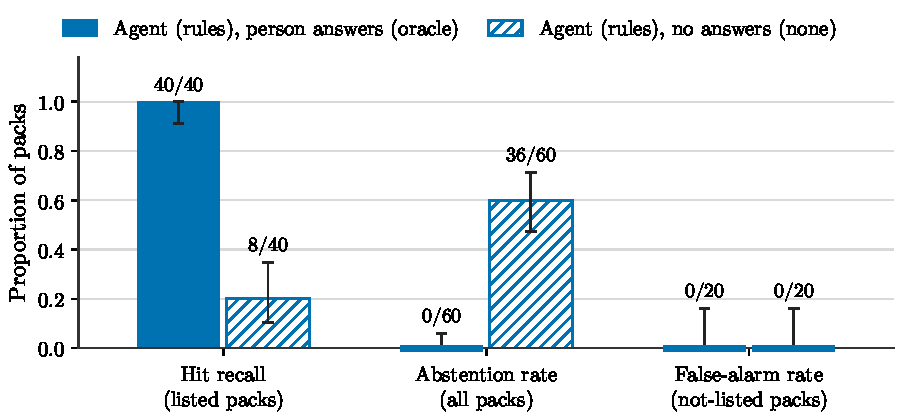
\includegraphics{fig_hitl_seed7.pdf}
\caption{Effect of the human answer for the agent with the rule planner, seed~7. Without answers
the agent abstains (\CANTV) on 36 of 60 packs, so hit recall falls while the false-alarm rate
stays at zero.}
\label{fig:eval-hitl}
\end{figure}

\begin{figure}[H]
\centering
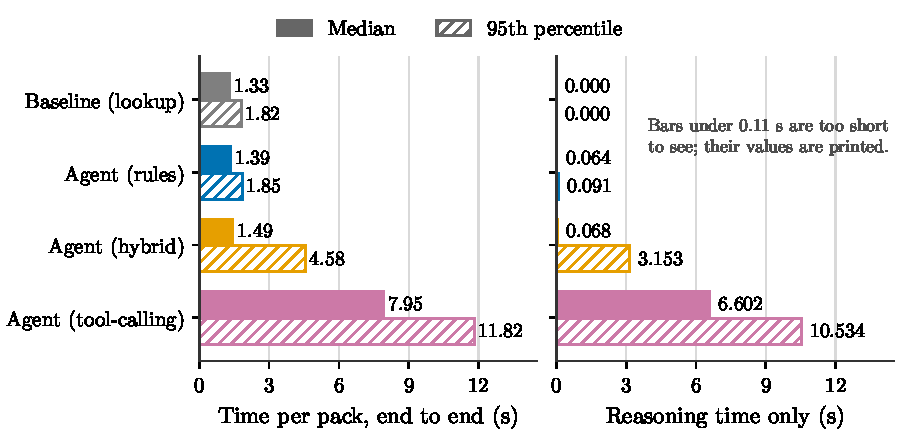
\includegraphics{fig_latency_seed7.pdf}
\caption{Time per pack on seed~7 ($n=60$, oracle). Left: end-to-end time (shared perception plus
reasoning). Right: reasoning time only. Solid bars are medians and hatched bars 95th percentiles.
The model calls of the hybrid and tool-calling planners set their tails.}
\label{fig:eval-latency}
\end{figure}

\section{Experimentation}

\begin{figure}[H]
\centering
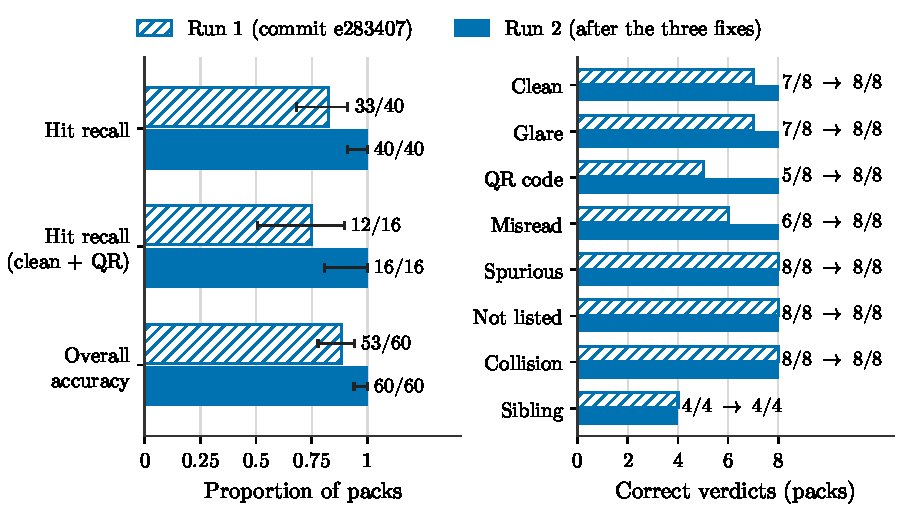
\includegraphics{fig_run1_run2.pdf}
\caption{Agent with the rule planner on seed~7 before (run~1) and after the three D25 fixes (run~2),
a person answering. Left: rates with Wilson 95\% intervals. Right: correct verdicts per scenario.
Labels on the right read run~1 $\rightarrow$ run~2. Run~1 is reported in full; because the fixes
were made after it, run~2 is not a blind test.}
\label{fig:exp-runs}
\end{figure}


\begin{table}[H]
\centering
\caption{Setup of the experiment}
\label{tab:exp-setup}
\small
\begin{tabularx}{\linewidth}{@{}>{\raggedright\arraybackslash}p{0.24\linewidth} X@{}}
\toprule
\textbf{Item} & \textbf{Setting} \\
\midrule
Arms & A: lookup script; B: agent, rule planner; C: agent, hybrid planner (\texttt{qwen2.5:3b} through
Ollama 0.17.7, temperature~0, JSON-schema output restricted to the allowed actions); D: agent, tool-calling planner (same model, native tool calls, tools limited by the rules; seed~7 only) \\
Human policy & Oracle (answers every question from the manifest) and none (every question skipped) \\
Packs & \res{ResN} rendered cartons per seed; seed~7 is the evaluation set, seed~1 the development
set on which thresholds were tuned \\
Held fixed & Perception output (read once per image and cached), index of \res{ResAlertCount}
alerts, verdict templates, verifier rules, loop bounds \\
Metrics & As defined in Section~\ref{sec:eval-metrics-and-evaluation-rubric} \\
Runs & Seed~7 twice (run~1 at commit \texttt{\RunOneCommit}, run~2 after decision D25); seed~1 once
with the run-2 code \\
Hardware & One Windows~11 laptop; OCR on the CPU; the model on the GPU in the seed-1 run (Ollama log), device not recorded for the seed-7 runs \\
\bottomrule
\end{tabularx}
\end{table}

\begin{figure}[H]
\centering
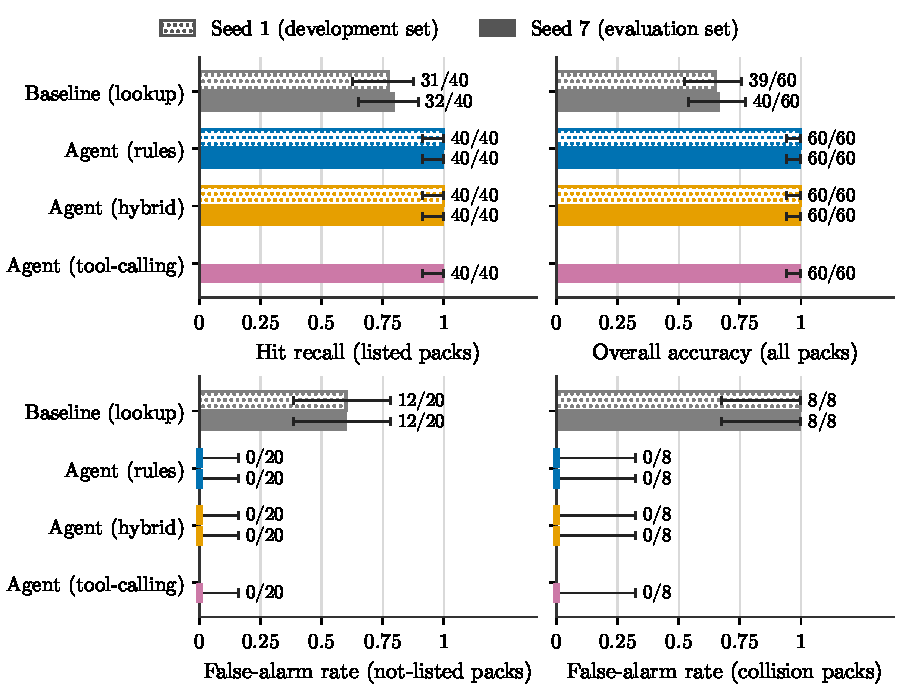
\includegraphics{fig_seeds.pdf}
\caption{Headline metrics on the development set (seed~1) and the evaluation set (seed~7), a person
answering, $n=60$ each. Labels give $k/n$ and whiskers are Wilson 95\% intervals. The agent arms give
the same counts on both sets; the lookup differs by one pack. The tool-calling arm was run on seed~7 only.}
\label{fig:exp-seeds}
\end{figure}

\section{Limitations and safety}

\begin{table}[H]
\centering
\caption{Failure modes, guardrails and where each guardrail is enforced}
\label{tab:lim-risks}
\footnotesize
\renewcommand{\arraystretch}{1.05}
\begin{tabularx}{\linewidth}{@{}>{\raggedright\arraybackslash}p{0.27\linewidth} >{\raggedright\arraybackslash}X >{\raggedright\arraybackslash}p{0.2\linewidth}@{}}
\toprule
\textbf{Failure mode} & \textbf{Guardrail} & \textbf{Enforced in} \\
\midrule
OCR reads a look-alike character with high confidence (\texttt{B} as \texttt{8}) & Variant search over look-alike pairs; \texttt{confirm\_char} question; an alarm needs a batch from QR, the person or two agreeing reads & \texttt{matching.py}, investigator, verifier R2 \\
Batch key shared by an unrelated product (collision) & Record-linkage grading on product, brand, dates and maker; a mismatch rejects the candidate & \texttt{grade()}, verifier R2 \\
Listed sibling batch one character away & Variant search runs even after an exact hit; \texttt{confirm\_batch} asks every look-alike position & investigator, decision D25 \\
LLM drafts before the variant search, is slow or unavailable, or returns invalid JSON & Action restricted to an allowed list; one send-back (R4); 15~s timeout, two attempts, rule fallback, 30~s circuit breaker & \texttt{llm.py}, investigator \\
Instructions hidden in pack or alert text & Text enters prompts only as JSON data; system message marks it untrusted; local endpoint only; model writes no user text & \texttt{llm.py}, \texttt{templates.py} \\
Wording that implies assurance or medical instruction & Banned-phrase check on every draft (R5); LLM thoughts redacted by the same check & verifier, \texttt{templates.py} \\
Loop or questions without end & At most 16 steps, 2 questions, 20 candidates, 1 send-back (R6) & \texttt{config.py}, verifier \\
Person skips a question, or a printed date disagrees with the entry & \CANTV{} with wording that sends the person to a pharmacist; \texttt{confirm\_field} question for a date (R7) & investigator, verifier \\
Lists stale, incomplete or malformed & \NLISTED{} states the lists loaded and the latest month and that it does not certify the medicine (R9); quarantine with reasons; rows keep source URL, SHA-256 and row number & verifier, \texttt{ingest.py} \\
Vision model reads a digit wrongly with high stated confidence & The reading is shown with its crop as a yes or no question and is never gate evidence alone; the look-alike search and the character question follow; 2 calls, 1 photo & \texttt{investigator.py}, verifier R2 \\
Hostile upload, or access to the laptop by others & 15~MB and 24 megapixel limits, 60~s deadline in a killable worker; server on localhost, pairing token for LAN and tunnel & \texttt{pack\_tools.py}, \texttt{server/app.py} \\
\bottomrule
\end{tabularx}
\end{table}
